%!TEX root = ../../fourthYearReport.tex


 
\paragraph{Work package 3 progress}

The progress for each task are described hereafter.

\subparagraph{Solving the local control problem (T3.3) (IIT: xxPM, UPMC: 3PM)}

During the fourth year, some improvements both in terms of parametrization and in terms of generic implementation have been brought to the whole-body control problem solving methods developed in CoDyCo.

\begin{itemize}
\item {Joint limit avoidance using an exogenous state description}
\end{itemize}
During year 4, IIT proposed a control laws ensuring the stabilization of a time-varying desired joint trajectory and joint limit avoidance (see Fig.~\ref{fig:icub leg limits} for an illustration of the limits on the leg) in the case of fully-actuated manipulators. The key idea is to perform a parametrization of the feasible joint motion space in terms of exogenous states $\xi$, in the form of $q(\xi) := \delta \tanh(\xi) + q_0$, where $q$ is the joint position, $\delta$ the range of feasible motion and $q_0$ its middle value. It follows that the control of the exogenous states allows for joint limit avoidance. One of the main outcomes of this work is that position terms in control laws are replaced by parametrized terms. Stability and convergence of time-varying reference trajectories obtained with the proposed method were demonstrated to be in the sense of Lyapunov. The introduced control laws were verified by carrying out experiments on two degrees-of-freedom of the torque-controlled iCub. This work led to a publication in Humanoid s 2016 \cite{charbonneau2016Humanoids}.

\begin{figure*}
   \begin{center}
    \includegraphics[width=0.4\textwidth]{images/iCub_joint_limits_leg.pdf}
    \caption{iCub leg setup used for the experiments. The red circles identify the hip and knee joints, while the white marks indicate joint limits. The green arrow shows the external force applied during experiments.}
    \label{fig:icub leg limits}
    \end{center}
\end{figure*}


\begin{itemize}
\item {Whole-body controller implementation}
\end{itemize}
As part of both WP1 and WP3, UPMC has pursued the generic implementation of an optimisation based whole-body controller named OCRA. See section~\ref{sec:OCRA}) for more details and \url{https://github.com/ocra-recipes} and \url{https://ocra-recipes.github.io/web} for online resources.

\subparagraph{Bootstrapping and validating the control approach in rigid world and compliant cases (T3.4) (TUD: 3.6PM, UPMC: 5.51PM, UB: xxPM, JSI: 1 PM, INRIA: 1.98PM)}

Over the fourth year, the bootstrapping of the whole-body control approach developed in CoDyCo has mostly been pursued in two directions. The first one is related to the learning of the dynamics for physical interactions. The second one is related to the adaptation of tasks and their proper activation for successful whole-body motions in contact.

\begin{itemize}
\item \textbf{Learning torque control}
\end{itemize}
TUD and INRIA, in collaboration with WP4, continued the collaboration on the topic of learning torque control in presence of multiple contacts, exploiting the force/torque and tactile sensors of iCub. Machine learning techniques were used to directly learn the mapping from both skin and the joint state to torques, using mixtures of contact models. Recently, the model was improved for torque control by addressing critical issues in learning from high-dimensional inputs, such as the artificial skin. It was demonstrated that it is possible to considerably reduce the dimensionality of the skin data preserving the information content of the contact position by using stacked auto encoders. A journal paper is currently in preparation. This technique will allow improving torque control in presence of multiple contacts (rigid and/or soft). This work is part of the PhD thesis work of Roberto Calandra on ``Bayesian Modeling for Optimization and Control in Robotics'' \cite{calandra2016PhD}.\\

\begin{itemize}
\item \textbf{Learning compliant contact models for interaction with non rigid environment}
\end{itemize}
As a part of T3.4, UB and TUD worked on developing a method to realize desired
contact normal forces between a robot's end-effector and its compliant
environment.  By using contact models, desired contact forces are converted to
desired deformations of compliant surfaces.  Therefore, the problem of
controlling compliant contact normal forces becomes the problem of controlling
surface deformations.  To study the performance of the proposed method in
practice, a series of experiments, including identification and control
experiments, were performed with a LWR KUKA manipulator.  During the
identification experiments, we estimated the contact models between the
robot's end-effector and two soft surfaces using least-squared linear
regression algorithm.  In control experiments, by using the estimated models,
we controlled the robot's motion in order to achieve various desired contact
normal forces for each surface.  We also studied the effects of updating model
parameters during control experiments using an online estimation method.  The
experiment results showed that desired forces can be achieved with some errors
while using the estimated model from identification experiments.  These errors
are decreased substantially by online adaptation of the contact model
parameters during control experiments.
%
\begin{figure}
  \centering
  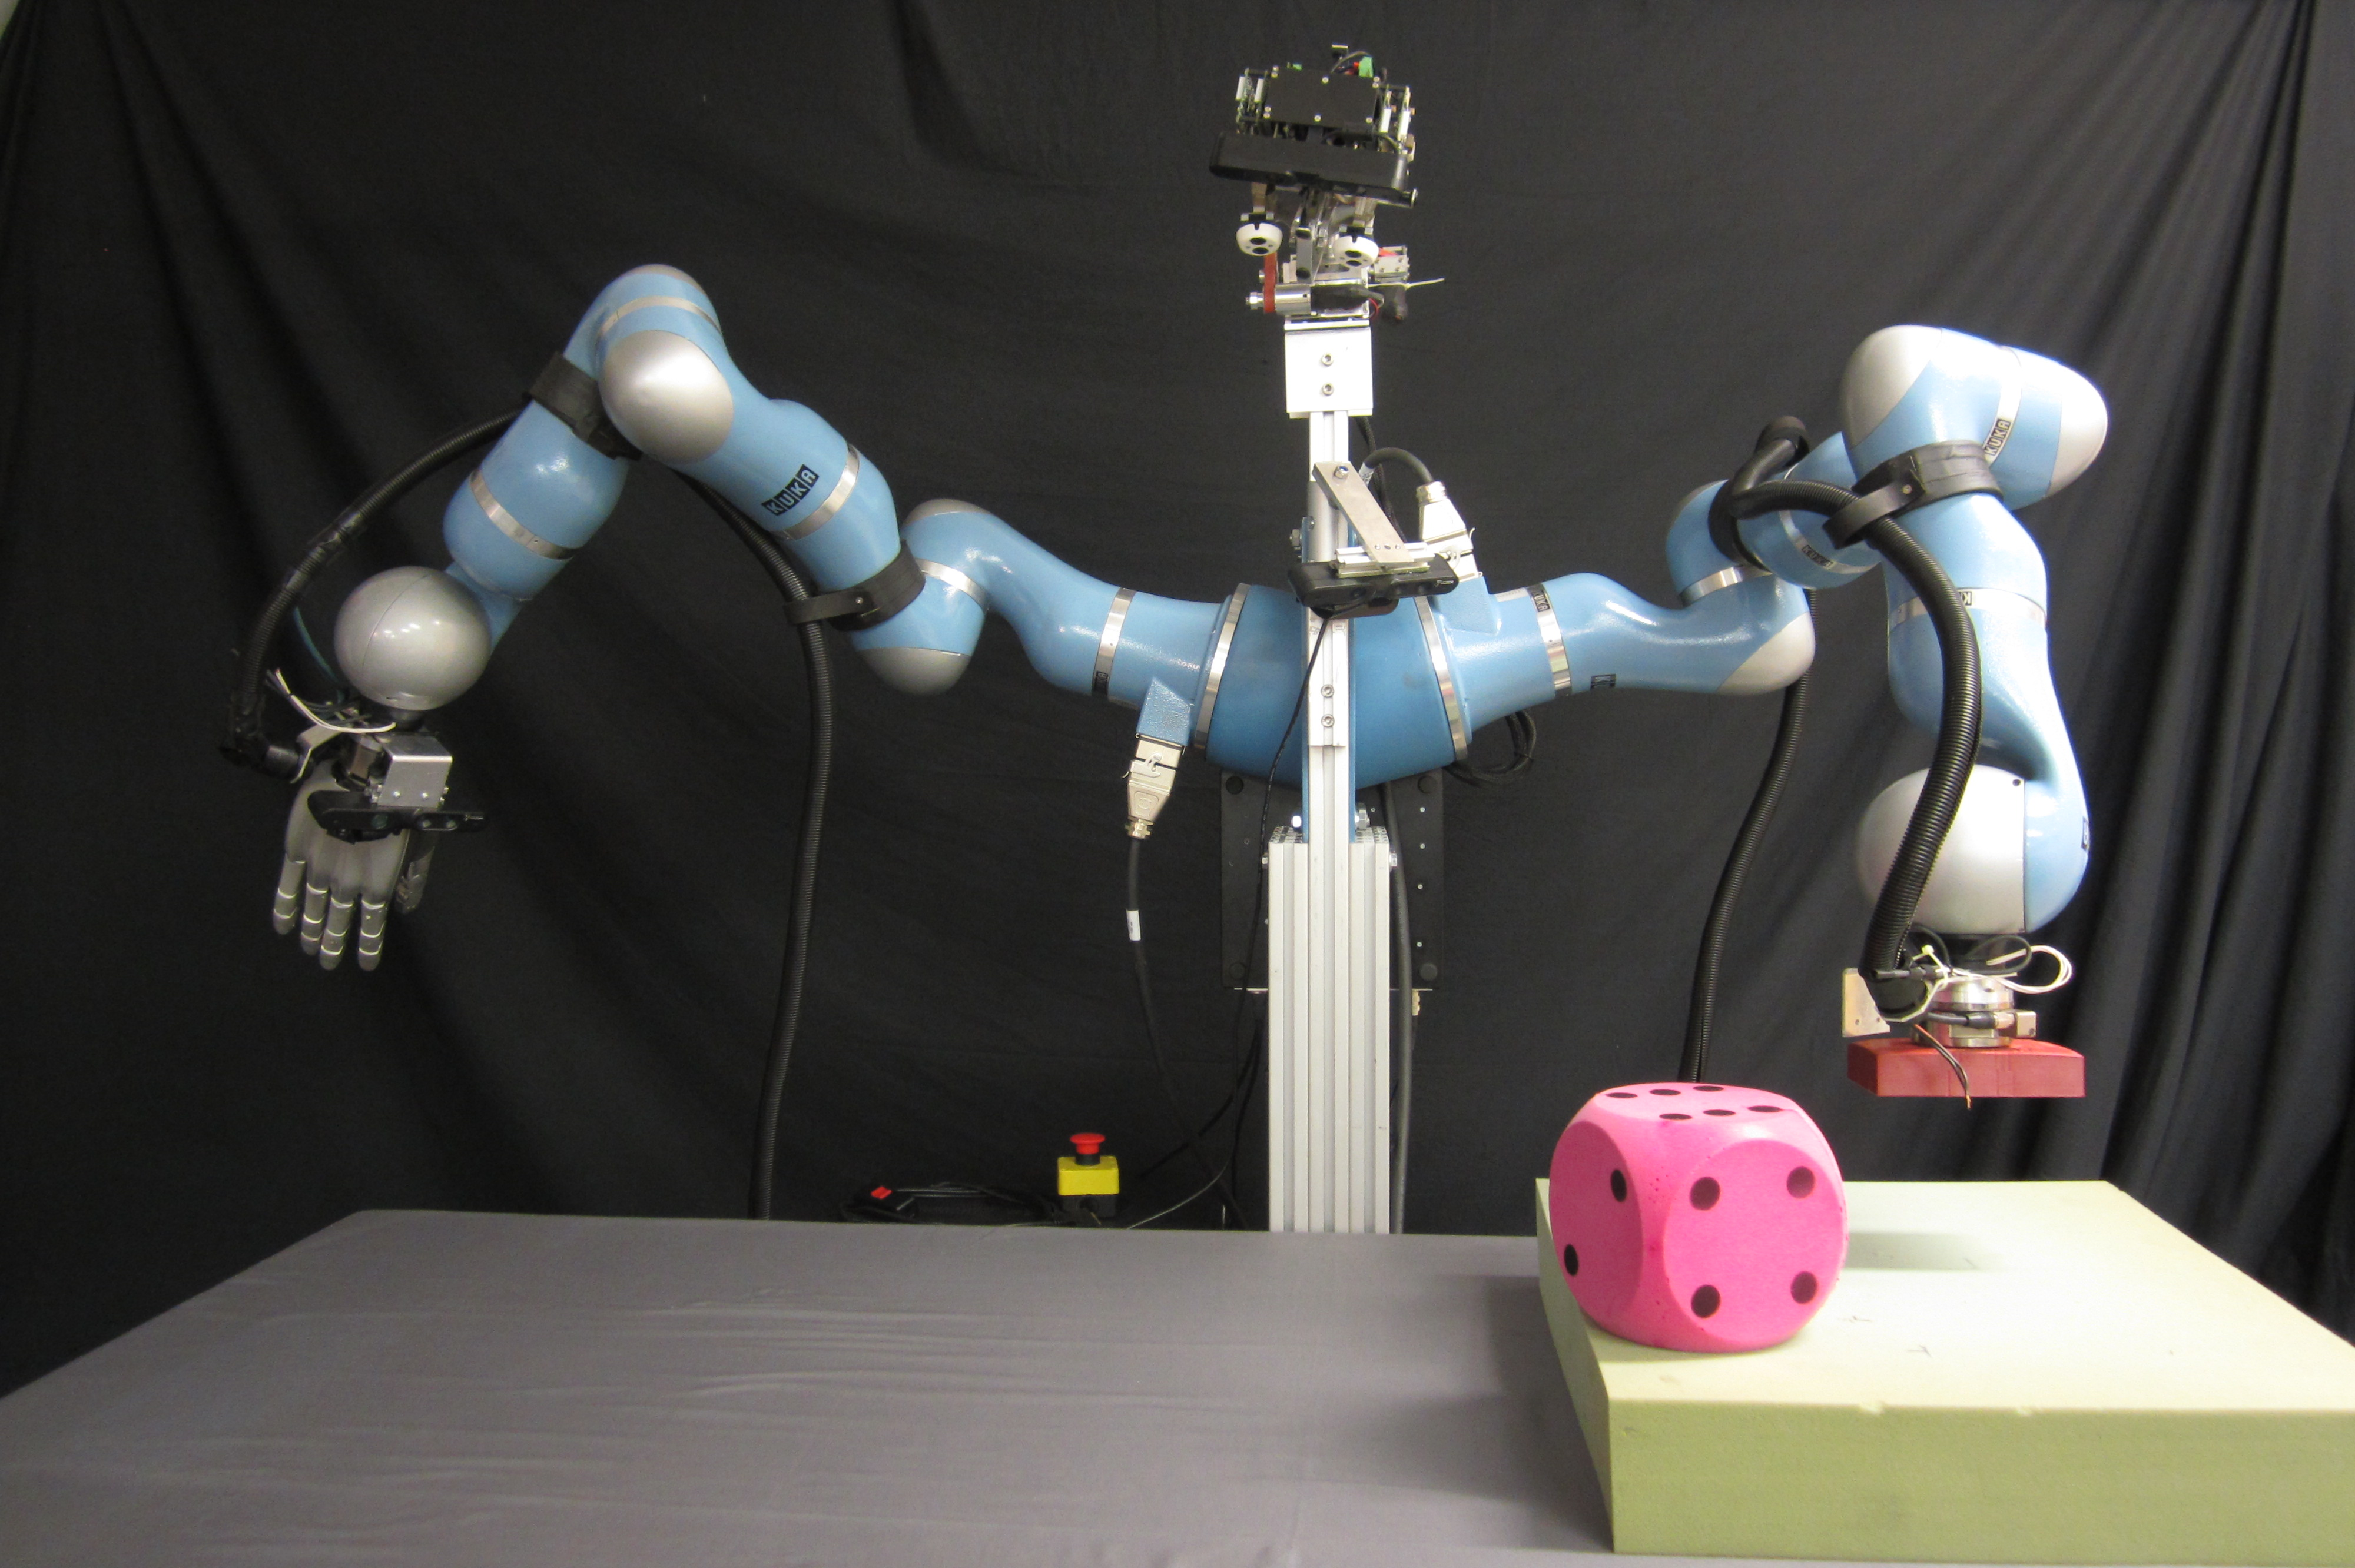
\includegraphics[scale=0.1]{images/Boris.jpg}
  \caption{KUKA LWR IV arms with two soft surfaces used in our experiments.}
  \label{Boris}
\end{figure}

\begin{itemize}
\item \textbf{Learning soft priorities}
\end{itemize}
INRIA also designed a multi-task prioritized controller with soft task priorities. The controller was first designed in \cite{Modugno2016} and applied to classical manipulators. In \cite{modugno2016learning} it was extended for whole-body movements. In the latter work, it was used to generate safe whole-body behaviors for iCub, reaching multiple goals and avoiding obstacles, with the guarantee that the generated behaviors were not violating the constraints of the platform. A software controller for iCub has been prototyped in Matlab then in C++.

\begin{itemize}
\item \textbf{Task compatibility optimization}
\end{itemize}
As part of both WP4 and WP3, UPMC has worked on improving its approach for task compatibility optimization. Modern control architectures employ multiple levels of control in order to decouple complex behaviors into manageable control problems. At the lowest level is reactive whole-body control, where joints torques are calculated at high frequency ($\sim1$kHz) given one or more tasks \cite{Khatib2004}. As presented in Deliverable~3.2~\cite{deliverable32}, the control problem can be written as a constrained convex optimization, where the objective function is a combination of task errors, and the constraints are the equations of motion, articulation and actuation limits, and contacts \cite{Salini2011, Saab2013, Bouyarmane2011}. Task errors are calculated as the difference between the current task state and its reference value. This reference value comes from the next level of task servoing. At this level, closed loop controllers are used to servo task trajectories using state feedback (PID) or Model Predictive Control (MPC) schemes at frequencies between $100$Hz and $10$Hz  \cite{Ibanez2014}, \cite{Koenemann2015}, \cite{Perrin2015}. These task trajectories are provided by higher-level open-loop planning which takes seconds to minutes, and generally combines operator expertise and automated planning algorithms \cite{Bouyarmane2012, Pham2014}. This control hierarchy of planning, servoing, and whole-body control is presented in Fig.~\ref{fig:control_diagram}.\\

Because each level in the control hierarchy is agnostic of the others by design, there is no guarantee that the planned task trajectories will be executed properly by the lower control layers~\cite{padois-HDR2016,ibanez_humanoidhandbook2016}. Furthermore, even though specific contexts such as non rigid contacts may be accounted for as described in Deliverable~3.2~\cite{deliverable32}, tasks may conflict with one another or be infeasible with the system constraints \cite{Bouyarmane2015, Wieber2017}. The end result is typically unstable or undesirable whole-body behaviors, and these tasks can be qualified as \textit{incompatible}. Prioritization techniques presented in Deliverable~3.2~\cite{deliverable32} use weighted sums\cite{Salini2011, Bouyarmane2011}, hierarchies~\cite{Saab2013,Escande2014, Dietrich2015} or a mix of both~\cite{liu-AutRob2015,liu-AutRobSI2015} to manage task incompatibilities at the whole-body control level, but are difficult to tune and only hide the problem. Moreover, tasks incompatibilities may be temporal and change over the course of the movement so applying static priorities may be overly restrictive. While the works presented in Deliverable~4.3~\cite{deliverable43} provide very powerful tools to reactively adapt priorities~\cite{Lober2015}, learn proper prioritizations~\cite{Modugno2016,modugno2016learning} or derive them from demonstrations~\cite{Paraschos_2017}, it seems obvious that well designed tasks should not need to be prioritized.\\

 Given that it is the task reference values which generate the incompatible control optima, an alternative to prioritization tuning is to modify the task trajectories supplied by planning and make them compatible as initially suggested in~\cite{Lober2014}. To do so, a feedback loop must be implemented, which measures the errors induced by incompatibilities and changes the task trajectories to reduce them. It should also take into account the servoing and whole-body control levels with all of their parameters, as well as the robot's dynamics and environment. Given the complexity of the proposed feedback loop, one solution is to use model-free Reinforcement Learning (RL) techniques to modify the trajectories through trial and error by minimizing some cost function using Black-Box Optimization (BBO) solvers \cite{Kober2013}.\\

\begin{figure}[!h]
\centering
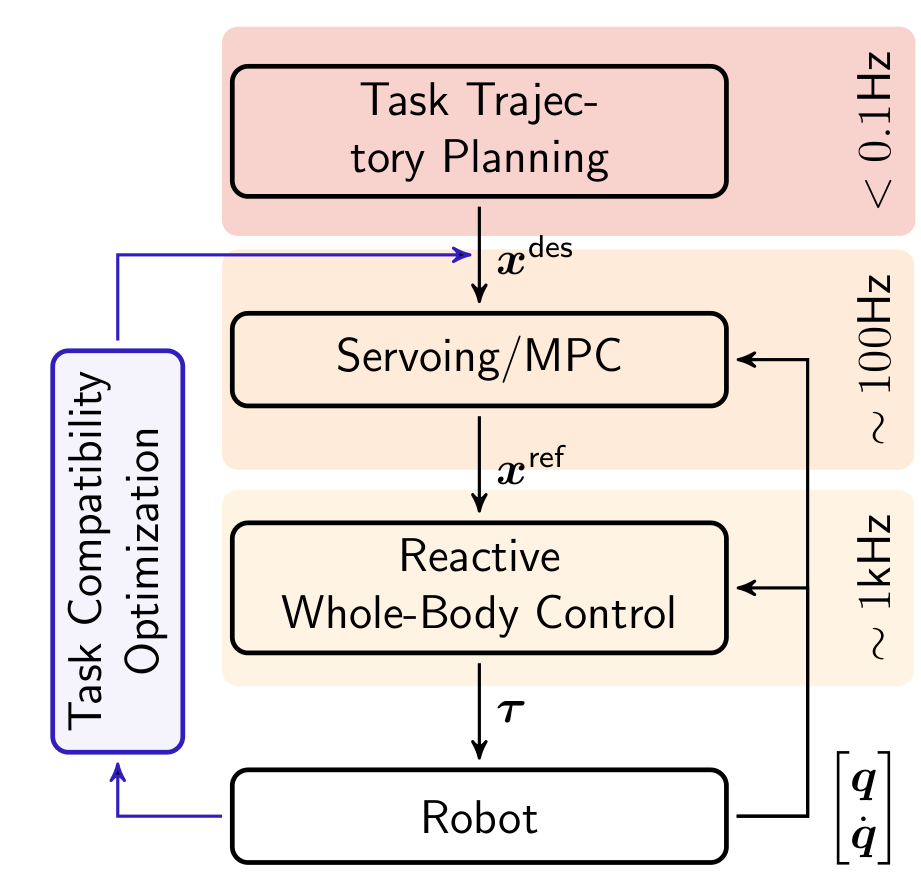
\includegraphics[width=0.4\textwidth]{images/control_pyramid.png}
\caption{A modern control hierarchy for highly redundant robotic systems, e.g. humanoid robots. At the lowest level is whole-body control, which determines the torques needed to accomplish a set of tasks. At the intermediate level, these tasks are controlled by the servoing/MPC level where task trajectory errors are compensated using state feedback. Finally the task trajectories are provided by high-level planning, which is usually a combination of operator expertise and automated planning. Each of these levels operates independently from one another and a feedback mechanism is needed to measure and compensate for tasks which are not executed as planned. This is the role of the Task Compatibility Optimization loop proposed in this work.}
\label{fig:control_diagram}
\end{figure}

The objective of the proposed approach is to establish the task compatibility optimization loop, shown on the left in Fig.~\ref{fig:control_diagram}, by iteratively improving task trajectories using RL. To do so, tasks trajectories are parameterized providing variables with which they can be modified. A generic task compatibility cost has been developed from simple principles which measures the incompatibility between one or more tasks and the robot's constraints. Using two common BBO solvers, this compatibility cost can be minimized by optimizing the task trajectory parameters. This task compatibility optimization has then tested on two typical muti-task scenarios. In the first scenario the relatively banal chore of reaching while balancing has be studied. While seemingly simple, reaching is a key ingredient in robot autonomy, which often requires parameter and gain tuning before done reliably. A performance comparison of two BBO solvers for this experiment has been performed to illustrate the generality of the framework. The second experiment explores the dynamically complex activity of moving from sitting to standing. This motion requires contact breaking and potentially unstable dynamic equilibrium to succeed. In both experiments a Center of Mass (CoM) task is used to maintain balance, and its trajectory is optimized to minimize the task compatibility cost. Through these two completely different motion scenarios, the proposed generic task compatibility optimization loop has shown to dramatically improve task achievement, without ever touching the low-level control parameters. These results extend the contributions \cite{lober-HUMANOIDS2014} and \cite{lober_IROS2015} both in terms of achieved performances and computational efficiency. This work and its potential use for the final demonstration are described with details in \cite{deliverable33} and was submitted for presentation at a robotics journal~\cite{lober2017RAL-IROS}.

\begin{itemize}
\item \textbf{Model Predictive stepping for robust balance}
\end{itemize}

As a part of both WP1 (see section~~\ref{sec:OCRA} for a list of associated software resources) and WP3, the predictive approach initially developed by A. Ibanez~\cite{ibanez2015Emergence} to preview the duration and placement of coplanar contacts has been implemented in the form of a client for OCRA using the iCub humanoid robot. Within a model-predictive control framework, the problem is formulated as a linearly constrained mixed-integer quadratic program (MIQP) which allows the determination over a preview horizon, of the optimal changes in the base of support of the robot with compatible CoM behaviour, subject to multiple constraints, while maximising balance and performance of a walking activity.

\subparagraph{Extra results in WP2/WP3: UPMC and JSI collaboration}

\begin{itemize}
\item \textbf{Adapting a reaching controller using the Speed-Accuracy trade-off}
\end{itemize}
As part of both WP2 and WP3, JSI, together with UPMC, continued the computational study where they try to describe the trade-off between the speed of motion, its accuracy and the muscular cost associated with the motion. They implemented a state-of-the-art deep reinforcement learning algorithm (DDPG) that is based on a deterministic policy gradient approach. DDPG allows more sample efficient learning, but is hard to tune in the context of a simulated reaching controller. They implemented the computations on the JSI cluster in Slovenia. Computations are currently running and the analyses remain to be performed.
    
\subparagraph{Deviations from workplan}  

The PM expenses for WP3 after one year of project are globally conform to the planned one.

%\emph{\color{red}[For work package 3 (UPMC) provide the following information:]}
%\begin{itemize}
%\item[-] \emph{\color{red}[A summary of progress towards objectives and details for each task;]}
%\item[-] \emph{\color{red}[Highlight clearly significant results;]}
%\item[-] \emph{\color{red}[If applicable, explain the reasons for deviations from Annex I and their impact on other tasks as well as on available resources and planning;]}
%\item[-] \emph{\color{red}[If applicable, explain the reasons for failing to achieve critical objectives and/or not being on schedule and explain the impact on other tasks as well as on available resources and planning (the explanations should be consistent with the declaration by the project coordinator) ;]}
%\item[-] \emph{\color{red}[a statement on the use of resources, in particular highlighting and explaining deviations between actual and planned  person-months per work package and per beneficiary in Annex 1 (Description of Work);]}
%\item[-] \emph{\color{red}[If applicable, propose corrective actions.]}
%\end{itemize}




